\section{Method}
\label{sec:method}

\subsection{Inventory Task}
\label{sec:inventory-task}

We use a finite-horizon, single-item lost-sales system with delayed and
potentially partial replenishment. Let $I_t$ denote on-hand inventory before
day-$t$ arrivals, $D_t$ realized demand, and $q_t\in\mathbb{Z}_{\geq 0}$ the
order selected from the public state. An earlier order $i$ of size $q_i$, due
on day $t$, arrives as $A_{i,t}\sim\operatorname{Binomial}(q_i,\rho_i)$ for its
quoted fill probability $\rho_i$ (and equals $q_i$ when $\rho_i=1$). The daily
dynamics are
\begin{align}
 A_t &= \textstyle\sum_{i:\tau_i=t} A_{i,t}, \quad
       I_t^{+} = I_t + A_t, \nonumber\\
 Y_t &= \min\{I_t^{+},D_t\}, \quad
       L_t = D_t-Y_t, \label{eq:inventory}\\
 I_{t+1} &= I_t^{+}-Y_t, \nonumber\\
 C_t &= c_p q_t+c_h I_{t+1}+c_s L_t+c_f\,\mathbb{1}[q_t>0]. \nonumber
\end{align}
Here $Y_t$, $L_t$, and $C_t$ are sales, lost sales, and operating cost. Demand
follows a scenario-specific Poisson or negative-binomial distribution. Under the
implementation's negative-binomial parameterization, mean $\mu_t$ and
dispersion $r_t$ imply success probability
$p_t=r_t/(r_t+\mu_t)$. Regime identity, future demand, supplier fill, and Oracle
state are hidden. The public observation contains the day, current inventory,
nominal pipeline inventory and due-day schedule, quoted lead time, last demand
and sales, costs, and the latest 14 days of realized history.

\subsection{Bounded Strategy Review and Daily Control}
\label{sec:bounded-control}

Given this task, ShiftMem treats memory reuse as bounded revision of a
three-parameter ordering strategy. The LLM acts only at scheduled or
change-triggered reviews, whereas a shared deterministic controller issues
daily orders. Figure~\ref{fig:architecture} summarizes this responsibility
split and the subsequent stages of delayed validation, lifecycle management,
and conditional retrieval.

\begin{figure*}[t]
  \centering
  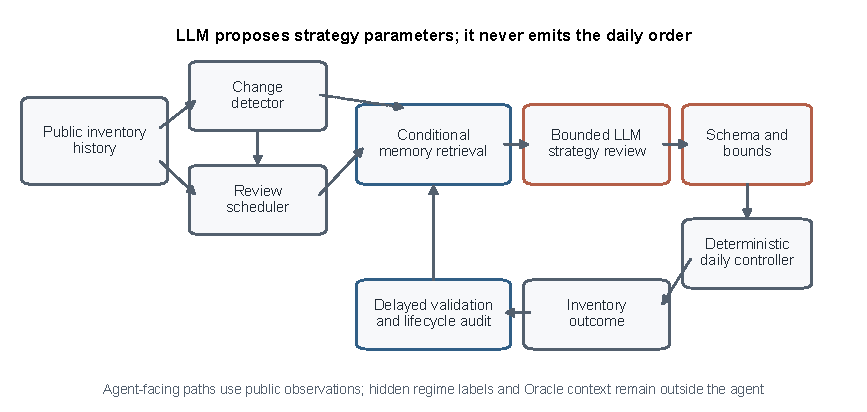
\includegraphics[width=\textwidth]{figures/figure_1_architecture.pdf}
  \caption{\textbf{Bounded strategy review and deterministic daily control.}
  Public inventory history drives the change detector and review scheduler. On
  an eligible day, method-specific memory is supplied to an LLM that may revise
  three bounded strategy parameters. Schema validation and deterministic
  projection precede the shared daily controller. Realized outcomes enter a
  delayed validation window and, for ShiftMem, an auditable lifecycle. The LLM
  neither emits daily orders nor observes hidden regime labels or Oracle state.}
  \label{fig:architecture}
\end{figure*}

The current strategy is
$\boldsymbol{\theta}_t=(w_t,k_t,b_t)$: a demand forecast window, safety-stock
multiplier, and lead-time buffer. Its initial value is $(14,1.2,1)$. At a review,
the LLM receives the public observation, current strategy, trigger, and up to
five retrieved experiences. It returns a structured proposal
$\widetilde{\boldsymbol{\theta}}_t$, cited experience IDs, model-reported
confidence, and a short reason. The cited IDs, model-reported confidence, and
reason are retained in the review log but do not directly set evidence-derived
lifecycle confidence. Unknown fields, malformed JSON, or citations to
experiences not supplied in the prompt cause one correction attempt. A second
failure retains the previous valid strategy.

Schema validation rejects proposals below the lower bounds. Remaining values
are projected first to the absolute bounds
$[1,60]\times[0,5]\times[0,14]$ and then to per-review changes
$\boldsymbol{\Delta}=(7,1,1)$:
\begin{equation}
 \theta_{t,j}^{\mathrm{new}}=
 \operatorname{clip}\!\left(
   \operatorname{clip}(\widetilde{\theta}_{t,j};\ell_j,u_j);
   \theta_{t,j}-\Delta_j,\theta_{t,j}+\Delta_j
 \right).
 \label{eq:strategy-projection}
\end{equation}
The projection limits abrupt changes and prevents the LLM from controlling the
action space directly.

The projected parameters determine daily orders through a deterministic
order-up-to controller. It uses the most recent $\min(w_t,14)$ available
demands to compute their mean
$\widehat{\mu}_t$ and sample standard deviation $\widehat{\sigma}_t$. With
quoted lead time $\ell_t$, nominal pipeline inventory $P_t$, and protection
horizon $h_t=\ell_t+b_t+1$, it sets
\begin{align}
 S_t &= \widehat{\mu}_t h_t
       + k_t\widehat{\sigma}_t\sqrt{h_t}, \label{eq:target}\\
 q_t &= \max\!\left\{0,
       \operatorname{round}\left(S_t-I_t-P_t\right)\right\}.
 \label{eq:controller}
\end{align}
Rounding follows the implementation's nearest-integer, ties-to-even rule. When
no history exists, the reset value of last demand, zero, is used. All compared
memory
methods share Eqs.~\eqref{eq:target}--\eqref{eq:controller}, the same strategy
bounds, and the same demand and calendar-indexed supply streams.

\subsection{Change-Triggered Review}
\label{sec:change-review}

A review occurs on days divisible by five, including initialization at day
zero, or on the day after a detector signal. An event-triggered review requires
more than three days since the previous review that included an event trigger. A
purely periodic
review neither starts nor resets this cooldown. Periodic and event triggers on
the same day are coalesced into one call. Thus the model cannot increase its own
review rate or alter the cooldown.

ShiftMem monitors public demand, lost sales, and quoted lead time with separate
two-sided Page--Hinkley detectors \citep{page1954continuous}. For observations
$x_n$ of one monitored variable, the running mean and one-sided accumulators are
\begin{align}
 \bar{x}_n &= \bar{x}_{n-1}+\tfrac{x_n-\bar{x}_{n-1}}{n}, \nonumber\\
 U_n &= U_{n-1}+x_n-\bar{x}_n-\delta, \nonumber\\
 G_n^{+} &= U_n-\min_{i\leq n}U_i, \label{eq:page-hinkley}\\
 V_n &= V_{n-1}+\bar{x}_n-x_n-\delta, \nonumber\\
 G_n^{-} &= V_n-\min_{i\leq n}V_i. \nonumber
\end{align}
After at least 10 samples, a signal is emitted when either statistic exceeds
$\lambda=48$, with $\delta=0.1$. Detector statistics reset after a signal. The
signal is an operational trigger, not an estimate of latent regime identity or
proof that a memory is invalid.

\subsection{Delayed Evidence and Memory Lifecycle}
\label{sec:lifecycle}

The memory unit is a valid bounded strategy revision, not a daily order. Each
valid review registers the new revision and separate reuse validations for its
cited experiences. If the review occurs on day $r$ with quoted lead time
$\ell_r$, validation starts at $a=r+\ell_r$ and uses the three complete days
$\mathcal{W}_r=\{a,a+1,a+2\}$. Define
\begin{equation}
 F_r=\frac{\sum_{t\in\mathcal{W}_r}Y_t}
           {\sum_{t\in\mathcal{W}_r}D_t},\quad
 L_r=\sum_{t\in\mathcal{W}_r}L_t,\quad
 \bar C_r=\frac{1}{3}\sum_{t\in\mathcal{W}_r}C_t,
 \label{eq:validation-metrics}
\end{equation}
where $F_r=1$ if total demand is zero. The deterministic verdict is
\begin{equation}
 z_r=\begin{cases}
 \mathrm{failure}, & F_r\leq0.80\ \lor\ L_r\geq1,\\
 \mathrm{support}, & F_r\geq0.95\ \land\ L_r=0\ \land\ \bar C_r\leq100,\\
 \mathrm{inconclusive}, & \text{otherwise}.
 \end{cases}
 \label{eq:validation}
\end{equation}
The window must be contiguous and complete. Because validation windows can
overlap and subsequent orders affect their outcomes, the resulting verdicts and
confidence values are operational lifecycle scores rather than causal estimates
of memory validity.

ShiftMem augments each experience with state
$s\in\{\mathrm{probation},\mathrm{active},\mathrm{dormant},\mathrm{invalid}\}$,
Beta evidence parameters initialized at $(\alpha,\beta)=(1,1)$, and support and
failure counts $(n_s,n_f)$. Its confidence and empirical utility are
\begin{equation}
 c=\frac{\alpha}{\alpha+\beta},\qquad
 u=\begin{cases}
 \dfrac{n_s}{n_s+n_f}, & n_s+n_f>0,\\
 0, & \text{otherwise},
 \end{cases}
 \label{eq:confidence}
\end{equation}
Support increments $(\alpha,n_s)$ by $(1,1)$. Failure increments
$(\beta,n_f)$ by $(\omega,1)$, where $\omega=2$ only when a reused experience
fails after a recorded related change and $\omega=1$ otherwise. Inconclusive
evidence leaves all four values unchanged. Detectors process each daily outcome
before due validations. A related signal on that outcome therefore activates
the post-change failure weight. A probationary
experience becomes active after at least two supports with $c\geq0.65$, and
becomes invalid after at least two failures with $c\leq0.35$. Failure returns an
active experience to probation, whereas the invalid state is terminal.

Each formal experience has an exact quoted-lead-time applicability condition;
demand context is not encoded as a stored applicability condition.
Three consecutive mismatching retrieval checks move an active or probationary
experience to dormant. A later condition match returns it to probation. These
are retrieval checks rather than elapsed days. Every transition is appended to
the lifecycle audit trail.

\subsection{Conditional Retrieval and Lexical Retrieval Baseline}
\label{sec:retrieval}

ShiftMem first excludes dormant, invalid, and condition-mismatched experiences.
It then ranks each eligible experience $m$ using
\begin{align}
 \operatorname{lexcos}(\xi,m)
 &=\frac{\sum_v n_v(\xi)n_v(m)}
 {\sqrt{\sum_v n_v(\xi)^2}\sqrt{\sum_v n_v(m)^2}}, \label{eq:lexcos}\\
 R_t(m)&=0.75\operatorname{lexcos}(\xi_t,m)+0.5c_m \nonumber\\
 &\quad{}+0.5^{a_m/30}+0.25u_m \nonumber\\
 &\quad{}-0.25\mathbb{1}[s_m=\mathrm{probation}]
 -0.5\mathbb{1}[V_m\cap\Delta V_t\neq\varnothing],
 \label{eq:retrieval-score}
\end{align}
where $\xi_t$ serializes the public observation and $\operatorname{lexcos}$
scores this serialization against the generated text of experience $m$. The tokenizer retains
each lowercase token matching \texttt{[a-z0-9\_]+}, and $n_v(\cdot)$ is its count.
$a_m$ is age in environment steps, $V_m$ is the experience-variable set, and
$\Delta V_t$ contains variables signaled within the previous 14 steps. Ties are
resolved by newer creation step and then ascending memory ID. The top five
experiences are supplied to the reviewer.

The comparison method, retained in code as \texttt{VectorMemory}, is an
implemented lexical retrieval baseline rather than an embedding model or vector
database. It stores every completed valid revision and ranks generated record
text only by Eq.~\eqref{eq:lexcos}, breaking ties by newer step and then
descending memory ID. Its ranker uses no applicability filter, lifecycle state,
evidence confidence, or change penalty.
Consequently, the experiment compares the implemented conditional-lifecycle
system with an implemented token-count cosine baseline under the same reviewer
and controller. It does not isolate any single ShiftMem component.

\subsection{Implementation and Comparison Boundaries}
\label{sec:method-boundaries}

The frozen implementation has several boundaries relevant to interpretation.
All three detector outputs can schedule reviews, but the model receives only a
generic event trigger rather than the variable and direction that fired. Direct
active-to-probation demotion and the changed-variable penalty require an exact
variable-name match between detector outputs and experience records. Only
demand satisfies this match. Quoted lead time instead controls applicability
through an exact stored condition. Because the public history contains 14 days,
$w_t>14$ is behaviorally indistinguishable in the controller. A pending reuse
verdict is not applied if its target becomes dormant or invalid before the
verdict is due.

Every memory method receives the same completed strategy-revision record. The
persisted record contains the projected strategy and validation metrics, while
the review log separately retains raw model output, reasons, model-reported
confidence, and cited experience IDs. Common record serialization also exposes
baseline experiences to the LLM with constant probation status and confidence
$0.5$. These fields do not affect lexical ranking but remain part of the tested
model-facing baseline. The primary comparison therefore concerns the two
implemented systems as deployed, not a mechanism-level ablation.
